\section{Arquitectura}

En la figura \ref{fig:arquitectura} se muestra el diagrama de la arquitectura propuesta con la que se trabajara para solucionar la problemática.

%En la figura \ref{fig:arquitectura} se describirá la arquitectura propuesta para la solución de la problemática.

\begin{figure}[htb]
	\centering
	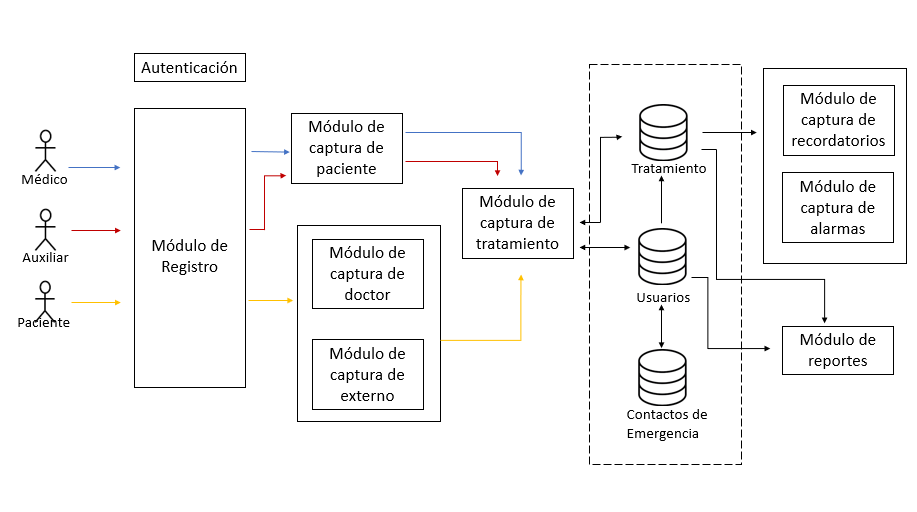
\includegraphics[width=0.8\textwidth]{images/cap2/Arquitectura}
	\caption{Arquitectura} \label{fig:arquitectura}
\end{figure}

Como podemos notar en la figura \ref{fig:arquitectura} se cuenta con cuatro actores que participaran en el sistema. Los cuales son :
\begin{itemize}
	\item Administrador: Dentro del sistema se le llama \textbf{Administrador} a la persona que esta encargada de ingresar los medicamentos a la base de datos, ya que estos serán los utilizados en los tratamientos del paciente.
	
	\item Paciente: Se le llama paciente a la persona que cuenta con un diagnostico generado por el \textbf{Médico} que se encuentra a cargo de su salud.\\
	Las acciones con las que cuentan son:
	\begin{itemize}
		\item Agregar el tratamiento medico.
		\item Modificar el tratamiento medico.
		\item Eliminar el tratamiento medico.
		\item Agregar médico.
		\item Modificar médico.
		\item Eliminar médico.
		\item Agregar externo.
		\item Modificar externo.
		\item Eliminar externo.
		\item Consulta de su tratamiento.
		\item Modificación de notificación.
		\item Agregar contactos de emergencia.
	\end{itemize}

	\item Médico: \\ \textbf{Médico} dentro del sistema es el profesional de la salud que se encarga del diagnostico del paciente y las acciones dentro del sistema son:
		\begin{itemize}
			\item consultar el total de pacientes que tiene.
			\item agregar un tratamiento medico a sus pacientes.
			\item modificar un tratamiento medico a sus pacientes.
			\item eliminar un tratamiento medico a sus pacientes.
			\item consultar el tratamiento medico de sus pacientes.
			\item consultar el historial medico de sus pacientes.
			\item agregar un paciente.
			\item modificar un paciente.
			\item eliminar un paciente.
		\end{itemize}

	\item Externo: El actor \textbf{Externo} nace de la necesidad de ayudar a los Pacientes que cuentan con poca o nula experiencia los dispositivos moviles o que por factores ajenas a la aplicación como son la de edad o alguna enfermedad les sea imposible utilizar la aplicación por si mismos\\
	Las acciones que tendra dentro de la aplicación son:
	\begin{itemize}
		\item Agregar Paciente.
		\item Modificar Paciente.
		\item Eliminar Paciente.
		\item Agregar Tratamiento medico.
		\item Modificar Tratamiento medico.
		\item Consultar Tratamiento medico.
		\item Modificar notificación
	\end{itemize}
\end{itemize}


\section{Módulos}
La arquitectura contara con los siguientes módulos:
\begin{itemize}
	\item Modulo de registro: Este modulo es el encargado de 
	
	
	\item Modulo de Autenticación:
	\item Modulo de captura de paciente:
	\item Modulo de captura de doctor:
	\item Modulo de captura de externo:
	\item Modulo de captura de tratamiento:
	\item Módulo de recordatorios:
	\item Módulo de alarmas:
	\item Módulo de reportes:
	
	
	
	
	
%	\item Módulo de Autenticación: El modulo encargado de verificar tu perfil y darte acceso a los módulos correspondientes.
%	\item Módulo captura de tratamientos: El modulo encargado de ingresar el tratamiento medico y lo asociara al perfil del paciente con la información correspondiente del tratamiento.
%	\item Módulo de recordatorios: Una vez que se paso por el modulo de \textbf{Captura de tratamiento} llegamos al modulo de recordatorios en donde se generaran los notificaciones a partir de la información obtenida del modulo de captura de tratamiento.
%	\item Módulo de alarmas: Este modulo es el encargado de cuando una notificación no haya sido silenciada esta se convierta en una alarma que le estará recordando al paciente tomar su medicamento.
%	\item Módulo de reportes: El modulo de reportes sirve para notificar al medico y al paciente que tan constante ha sido con su tratamiento.
%	\item Módulo de estadísticas: 
\end{itemize}

%\textbf{Módulo Autenticación: } Este modulo es el encargado de verificar cual es tu perfil y darte acceso a los módulos correspondientes.
%
%\textbf{Módulo captura de tratamientos: }Este módulo es el encargado de ingresar el tratamiento medico que expida el medico y asociar al perfil todos los detalles como lo son, los medicamentos, la dosis.
%
%\textbf{Módulo de recordatorios: }Este módulo es el encargado de crear los recordatorios para el tratamiento medico asociado al perfil.
%
%\textbf{Módulo de alarmas: }Este módulo se encargara de gestionar a tus contactos de emergencia y te permitirá editar convertir los recordatorios a alarmas de aquellos medicamentos que sean muy importantes.
%
%\textbf{Módulo de reportes: }Este módulo generara un reporte en pdf que mostrara el tratamiento medico actual.

%\textbf{Módulo de estadísticas:} Este módulo permitirá la visualización de información medica del paciente y de los medicamentos que toma.